\documentclass[12pt]{article}
\usepackage[english]{babel}
\usepackage[utf8x]{inputenc}
\usepackage[T1]{fontenc}
\usepackage{scribe}
\usepackage{listings}
\usepackage{graphics, graphicx}
\usepackage{enumerate}
\usepackage{enumitem}
\usepackage{tcolorbox}
\usepackage{adjustbox}
\usepackage{mathtools}
\usepackage{amsmath}
\usepackage[edges]{forest}
\DeclarePairedDelimiter{\ceil}{\lceil}{\rceil}

\newcommand{\forceindent}{\leavevmode{\parindent=1.3em\indent}}
\newcommand{\dbt}{\forceindent \forceindent}
\graphicspath{ {./images/} }

\CourseName{Comtemporary Algorithms T.II/2019-20}
\Scribe{Kanokpon \& Kanokpon}
\Lecturer{Dr. Kanat Tangwongsan}
\LectureNumber{4}
\LectureDate{15 January 2020}
\LectureTitle{Nearest Neighbours II}

\lstset{style=mystyle}

\newlist{steps}{enumerate}{1}
\setlist[steps, 1]{label = Step \arabic*:}

\begin{document}
\MakeScribeTop

\underline{Input:} a collection $D=\{P_1,P_2, P_3,...P_n\} \subset \chi$ of $n$ points

\dbt a dist function $d: \chi * \chi \to \mathbb{R}_+ \cup \{0\}$\\

\underline{Query:} given a query $q \in x$ find (all)points near $q$\\

Two ingredients in the above formulation:
\begin{enumerate}
	\item a (dis)aimilarity measure.
	\item an efficient d/s \& algo baseline: $O(n)$ probes
\end{enumerate}
Similarity = -dist

\section{Euclidian distance ($l_2$ distance)}

Measure of dissimilarity
\begin{align*}
	\vec{x},\vec{y} &\in \mathbb{R}^d\\
	d(\vec{x}, \vec{y}) &= ||x-y||_{l_2} &-\text{known as $l_2$ norm}\\
	&=\sqrt{(\vec{x}-\vec{y})^T (\vec{x}-\vec{y})}\\
	&=\sqrt[2]{\sum_{i=1}^{d}(x_i-y_i)^2}\\
\end{align*}
\section{General Norms ($l_p$ norms)}
\begin{align*}
\text{For } p&>0, ||x-y||_{l_p} = \sqrt[p]{\sum(x_i-y_i)^p}\\
p&=0 : \text{How many non-zero coordinate $||\vec{x}-\vec{y}||_{l_0}$}\\
p&= \infty : \text{max $x_i - y_i$}\\
p&=1 : \text{Manhattan Dist}
\end{align*}
\section{Jaccard}
How similar are these two sets?
\begin{align*}
	S,T &\subseteq u\\
	J(S, T) &= \frac{|S \cap T|}{S \cup T}
\end{align*}
\section{Cosine Similarity}
Cosine similarity: $
\frac{\langle x,y \rangle}{||x||\: ||y||}
$\\
Angular distant: $\cos^{-1}(\frac{\langle x,y \rangle}{||x||\: ||y||})$

\section{Low-dimensional Space}
	
		\subsection{d = 1}
		\begin{itemize}
			\item balance search tree
			\item sorted array
			\item $O(\log n)$ time/query
			\item $O(n)$ space
			\item $O(n\log n)$ preprocessing
		\end{itemize}
		\subsection{d = 2}
		\begin{itemize}
			\item Voronoi
			\item KD tree
			\item OCT tree
		\end{itemize}
	
\textbf{Voronoi}

For each point in $D$, construct (and store) the region that contains all of its closest neighbors
$$
VR_i = \{ x\in \chi | d(x_i,p_i)\leq d(x_j, p_j) \forall j \neq i \}
$$
\begin{itemize}
	\item $n \log n$ time to build
	\item $O(n)$ space
	\item $O(\log n)$ query(via point location)
\end{itemize}

\textbf{KD trees}
\begin{itemize}
	\item space partitioning technique
	\item alternate b/w vertical and horizontal cuts
	\begin{itemize}
		\item find a median split point
		\item recurse until 1 point
		\item yield a BST
	\end{itemize} 
\end{itemize}
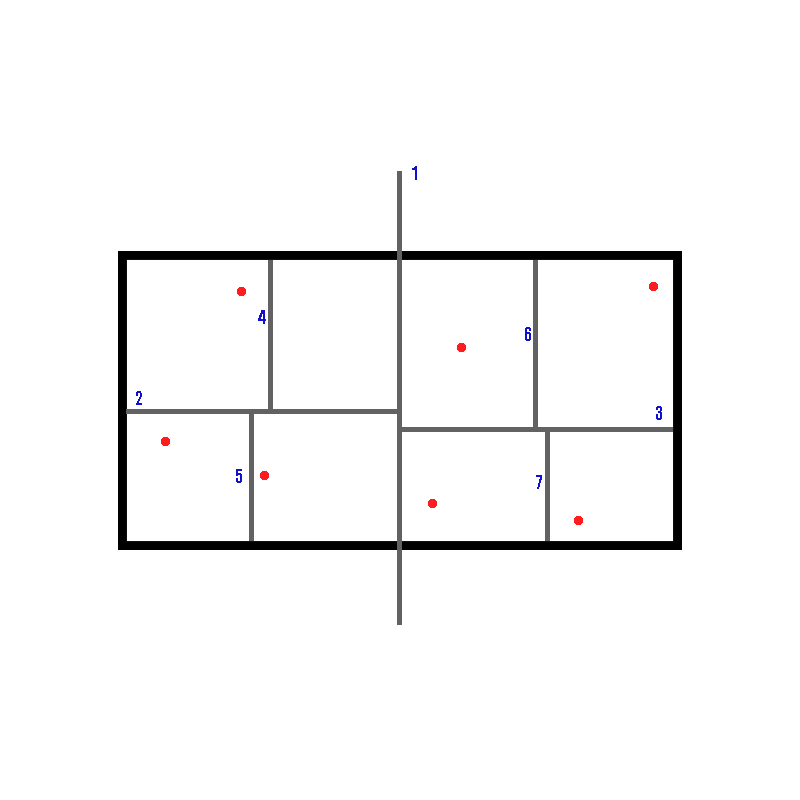
\includegraphics{calgo.png}\\
\begin{forest}
	for tree={grow=south,
	circle, draw, minimum size=3ex, inner sep=1pt,
	s sep=7mm
	}
	[1
		[2
			[4][5]
		]
		[3
			[6][7]
		]
	]
\end{forest}\\\\
Rectangle query (range query)

find all points of $D$ in $D \cap R$\\

Start at root \& recurse
\begin{enumerate}[align=left, labelwidth=1ex, start=1,label={case \roman*:}]
	\item This node region $\subseteq R$\\
	return everything in this subtree
	\item this node's region $\cap R = \emptyset$\\
	return $\emptyset$
	\item this node's region $\cap R \neq \emptyset$\\
	recurse \& return the union of the answers from2 subtrees
\end{enumerate}

Total query cost = $\overbrace{\text{\# nodes visited}}^{O(\sqrt{n})} $ + $\overbrace{\text{\# pts reported}}^{s}$

\underline{Observation:} \#nodes visited $\leq$ \# nodes where regions are intersected by an edge of $R$\\
\begin{align*}
&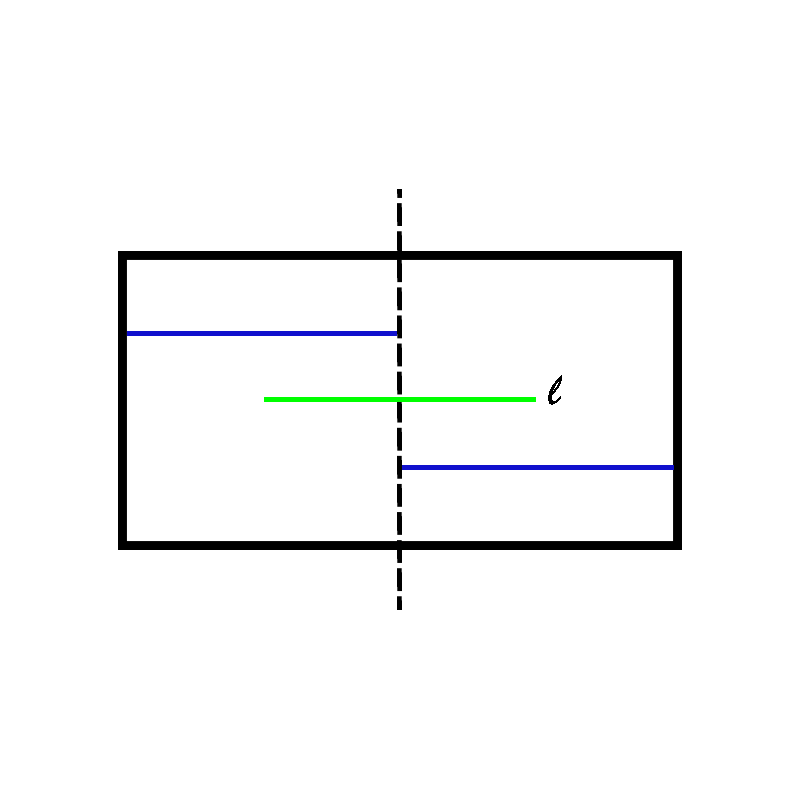
\includegraphics{calgo1.png} 
\end{align*}

$R$ has 4 edges. Consider one of them names $l$ (others are symmetric)
\begin{itemize}
	\item $l$ intersects $\leq3$ nodes regions.
	\item continue to be present in $\leq2$ regions.
	\item The recursion turns 1 into 4 regions .
\end{itemize}
\begin{align*}
\Rightarrow f(n)&\leq 3 + 2f(\frac{n}{4})\\
f(n) &\leq O(\sqrt{n})
\end{align*}
\begin{itemize}
	\item space: $1+2+2^2+...+2^{\log n} = O(n)$
	\item preprocessing: $O(n\log n) \Leftarrow n\log n$(sorting) + $\left[T(n)=2T(n/2)+O(n)\right]$
	\item query: $O(\sqrt n + s)$
\end{itemize}
\subsection{d > 2}
\begin{itemize}
	\item Voronoi
	\begin{itemize}
		\item has $\Omega (n^{\ceil{\frac{d}{2}}})$ "sites"
			\item $O(n^d)$ space and $(d+\log n)^{O(1)}$ time to query
	\end{itemize}
	\item KD-tree
	\begin{itemize}
		\item query: $O(dn^{1-\frac1d}+s)$ [still prefer if $d\leq50$]
	\end{itemize}
\end{itemize}
\section{Aim}
\begin{enumerate}[align=left, labelwidth=1ex, start=1,label={\#\arabic*}]
	\item Dimensionality reduction JL
	\item Hash \& Approximate LSH
	\item Data-dependent schemes PCA
\end{enumerate}

\subsection{Johnson-Lindenstrauss}

JL-Lemma states that any $n$ points in high dimensional euclidian space can be mapped onto $k$ dimensions where $k \geq O(\frac1{\varepsilon^2}\log n )$ without distorting the euclidian distance between any two more than a factor 

Find a mapping $f: u^D \to V^d$ s.t. (embedded space) $d_V(f(x), f(y)) \in (1\pm\varepsilon)d_u(x,y)$
\begin{enumerate}[align=left, labelwidth=1ex, start=1,label={Lemma \arabic*}]
	\item \textbf{(Johnson-Lindenstrauss)}\\
	Let $0<\varepsilon<\frac12$ Given any set of points\\
	$\{p_1, p_2, \dots, p_n \}\subseteq \mathbb{R}^D$ there exists a mapping $f: \R^D\mapsto\R^k$\\
	with $k=O(\frac{1}{\varepsilon^2}\log n)$ such that $||f(p_i)-f(p_j)||_2^2\in (1\pm \varepsilon)||p_i-p_j||_2 ^2$
	\begin{align}
	M_X
	&=\left[
	\begin{matrix}
	&M_1\\
	&\vdots&\\
	&M_k&
	\end{matrix}
	\right]_{K\times D} 
	\left[
	\begin{matrix}
	x_1\\
	\vdots
	\\
	x_n
	\end{matrix}
	\right]
	&;M_{n,i}\sim N(0,1)
	\\
	&=\left[
	\begin{matrix}
	\langle M_1, x \rangle\\
	\vdots\\
	\langle M_k, x \rangle\\
	\end{matrix}
	\right]\\
	f(x) &= \frac{1}{\sqrt k}M_x
	\end{align}
	\item \textbf{(Distributional JL)}
	
	Let $0 < \varepsilon < \frac12$ If $f$ is constructed\\
	 per above with $k=8\varepsilon^{-2}\ln\frac2\delta$ with $x \in\R^D$, with $||x||_2=1$ then\\ $\Pr[||f(x)||_2^2\in1\pm\varepsilon] \geq 1-\delta$
	
	\begin{align}
	\Delta &= f\left( \frac{\overbrace{P_i-P_j}^x}{||p_i-p_j||} \right)\\
	&=\frac1{\sqrt k}M(\cdots)\\
	&=\frac{1}{||p_i - p_j||}(f(p_i) - f(p_j))\\
	||\Delta||^2_2&=\frac1{||p_i-p_j||_{l2}^2}||f(p_i)-f(p_j)||^2_{2}\\
	\\
	\text{Let }x&= \frac{P_i-P_j}{||p_i-p_j||}\\
	||x||_{2}&=1\\
	\frac{||f(p_i)-f(p_j)||^2_{2}}{||p_i-p_j||^2_{2}}&=||\Delta||^2_{2}\in 1\pm\varepsilon\quad\text{Proved Lemma 1}\\
	\\
	\text{Let }\delta &= \frac2{n^2}\\
	k&=\frac{8}{\varepsilon^2}\ln\frac2{\frac2{n^2}}\\
	&=\frac8\varepsilon^2\ln{n^2}
	\end{align}
	for pair $(i, j), \Pr \left[\Delta \notin 1 \pm \varepsilon\right] < \frac1{n^2}$\\
	$\big(\begin{smallmatrix}
		n \\
		2
	\end{smallmatrix}\big)$
	pairs total $\Rightarrow \Pr \left[\text{at least one has } \Delta \notin 1\pm \varepsilon \right]$\\
	$\begin{smallmatrix}
	\text{union} \\
	\text{bound}
	\end{smallmatrix} < (\frac n{2})\frac{1}{n^2} \leq \frac{1}{2}$\\
	\textbf{w.p.} $\geq \frac{1}{2}$, all pairs are good
	
	$A(x) = \frac1{\sqrt k}M_x$
	
	matrix $M_{K \times D}, N_{i,j}~(0,1)$
	
	Let $0<\varepsilon < \frac1{2}$ If $A$ is as defined above with $k=8\varepsilon \ln (\frac2{\delta})$ and $x \in \mathbb{R}^D$ with$||x||_2 = 1$\\
	then, $\Pr\left[||A(x)||^2_2 \in 1 \pm \varepsilon \right] \geq 1-8$
	
	$N(\mu, \sigma^2)$ mean $\mu$ and variance $\sigma^2$\\
	pdf: $f(x) = \frac{1}{2\pi\sigma}e^{\frac{(x-\mu)^2}{2\sigma^2}}$\\
	then:
	\begin{eqnarray*}
	CG_1&\sim& N(c\mu_1, c^2\sigma_1^2) \\
	G_1 + G_2 &\sim& (\mu_1+\mu_2, \sigma_1^2, \sigma_2^2)\\
	A(x)&=&\left[
	\begin{matrix}
		M_1\\
		\vdots\\
		M_k
	\end{matrix}
	\right]
	\left[
	\begin{matrix}
		x_1\\
		\vdots
		\\
		x_D
	\end{matrix}
	\right] = \frac{1}{\sqrt{k}}
	\left[
	\begin{matrix}
		<M_1x>\\
		<M_2x>\\
		\vdots
		\\
		<M_kx>
	\end{matrix}
	\right]
	\begin{matrix}
		-y_1\\
		-y_2\\
		\vdots
		\\
		-y_K
	\end{matrix}\\
	y_i &=& \left[G_1, G_2,\dots, G_2\right]
	\left[ \begin{matrix}
		x_1\\
		\vdots
		\\
		x_D
	\end{matrix}
	\right]
	= \sum^D_{j=1}G_jx_j, \text{where $G_j \sim N(0,1)$}\\
	y_i &\sim& N(0, \underbrace{||x||^2_2}_{=1}) = N(0,1)\\
	Z &=& ||A(x)||^2_2 = A(x)^TA(x) = \frac{1}{k} \sum y_i^2 \to \text{chi$^2$ disttribution with $k$ doF}\\
	\mathbb{E}\left[Z\right] &=& \frac{1}{k}\sum \mathbb{E}\left[y_i^2\right] =1 = ||x||_2^2\\
	\mathbb{E}\left[||A(p)-A(q)||_2^2\right] &=& \mathbb{E}\left[||A(p-q)||_2^2\right] = ||p-q||_2^2\\\\
	\Pr\left[Z > 1+\varepsilon \right] \forall t&>&0\\
	&=& \Pr\left[e^{tkz} \geq e^{tk(1+\varepsilon)}\right]\\
	&\leq& \frac{\mathbb{E}\left[e^{tkz}\right]}{e^{tk(1+\varepsilon)}} \forceindent ;e^{tkz} = e^{tk\frac{1}{k}\sum y_j^2} = \Pi e^{ty_j^2}\\
	&=& \Pi \frac{\mathbb{E}\left[e^{ty_j^2}\right]}{e^{tk(1+\varepsilon)}}
	\end{eqnarray*}

	\textbf{claim1: } $\mathbb{E}\left[e^{tG^2}\right] = \frac1{\sqrt{1-2t}}$ for $t < \frac12$\\
	\textbf{claim2: } $\frac{1}{e^t\sqrt{1-2t}} \leq e^{\frac{t^2}{1-2t}}$ 
	\begin{eqnarray*}
	&=& \left(\frac{1}{e^{t(1+\varepsilon)}\sqrt{1-2t}}\right)^k\\
	&\leq& exp\left\{ \frac{kt^2}{1-2t} - k+\varepsilon\right\}\\
	\text{use } t &=& \frac{\varepsilon}{4} \leq e^{\frac{-k\varepsilon^2}{8}}\\
	\text{Recall } \varepsilon &<& \frac12\\
	\text{choose } k &=& \frac{8}{\varepsilon^2}\left(\frac{2}{\delta}\right) = \frac{\delta}{2}\\
	\Pr\left[Z < 1-\varepsilon\right] &<& \frac{\delta}{2}
	\end{eqnarray*}
\end{enumerate}

\end{document}
